\section{실험}
\label{sec:experiments}

\begin{table*}[t!]

\resizebox{\textwidth}{!}{
\begin{tabular}{@{} l l l c c c c c c c c @{}}
\toprule

\multirow{2.5}{*}{\textbf{모델}} & \multirow{2.5}{*}{\textbf{예측 공간}} & \multirow{2.5}{*}{\textbf{학습 목적 함수}} & \multicolumn{2}{c}{\textbf{가격 시계열 예측}} && \multicolumn{2}{c}{\textbf{수익률 예측}} && \multicolumn{2}{c}{\textbf{변동성 예측}} \\
\cmidrule(lr){4-5} \cmidrule(lr){7-8} \cmidrule(lr){10-11}

& & & IC ($\uparrow$) & RankIC ($\uparrow$) && IC ($\uparrow$) & RankIC ($\uparrow$) && MAE ($\downarrow$) & R$^2$ ($\uparrow$) \\
\midrule

Direct-AR       & 연속형 & 평균제곱오차 (MSE)  & 0.0212 & 0.0149 && 0.0416 & 0.0399 && 0.0565 & 0.1608 \\
Prob-AR         & 연속형 & 음의 로그가능도 (NLL) & 0.0179 & 0.0102 && 0.0356 & 0.0329 && 0.0464 & 0.1383 \\
\midrule

Kronos-Parallel & 이산형   & 교차 엔트로피             & 0.0345 & 0.0226 && 0.0529 & 0.0505 && 0.0461 & 0.1784 \\
\textbf{$\text{Kronos}_{small}$} & \textbf{이산형}   & \textbf{교차 엔트로피}    & \textbf{0.0431} & \textbf{0.0254} && \textbf{0.0665} & \textbf{0.0622} && \textbf{0.0384} & \textbf{0.2490} \\
\bottomrule
\end{tabular}
}
\centering
\caption{
    Kronos의 아키텍처 선택을 세분화해 분석한 제거 연구.
    우리는 서로 다른 \textbf{예측 공간}(연속형 vs. 이산형)과 이에 대응하는 \textbf{학습 목적 함수}를 대상으로 하는 변형들과 우리 모델을 비교한다.
    \textit{Direct-AR}은 표준 회귀 기준선 역할을 한다.
    \textit{Prob-AR}은 연속 공간에서 확률적 모델링의 이점을 평가한다.
    \textit{Kronos-Parallel}은 서브토큰을 동시에 예측함으로써 우리의 순차적 서브토큰 설계를 제거한 변형이다.
    % 화살표($\uparrow$/$\downarrow$)는 선호되는 방향을 나타낸다.
    최상의 결과는 \textbf{굵게} 표시한다.
}
\label{tab:ablation_study_refined}
\end{table*}

\begin{figure*}[htbp]
    \centering
    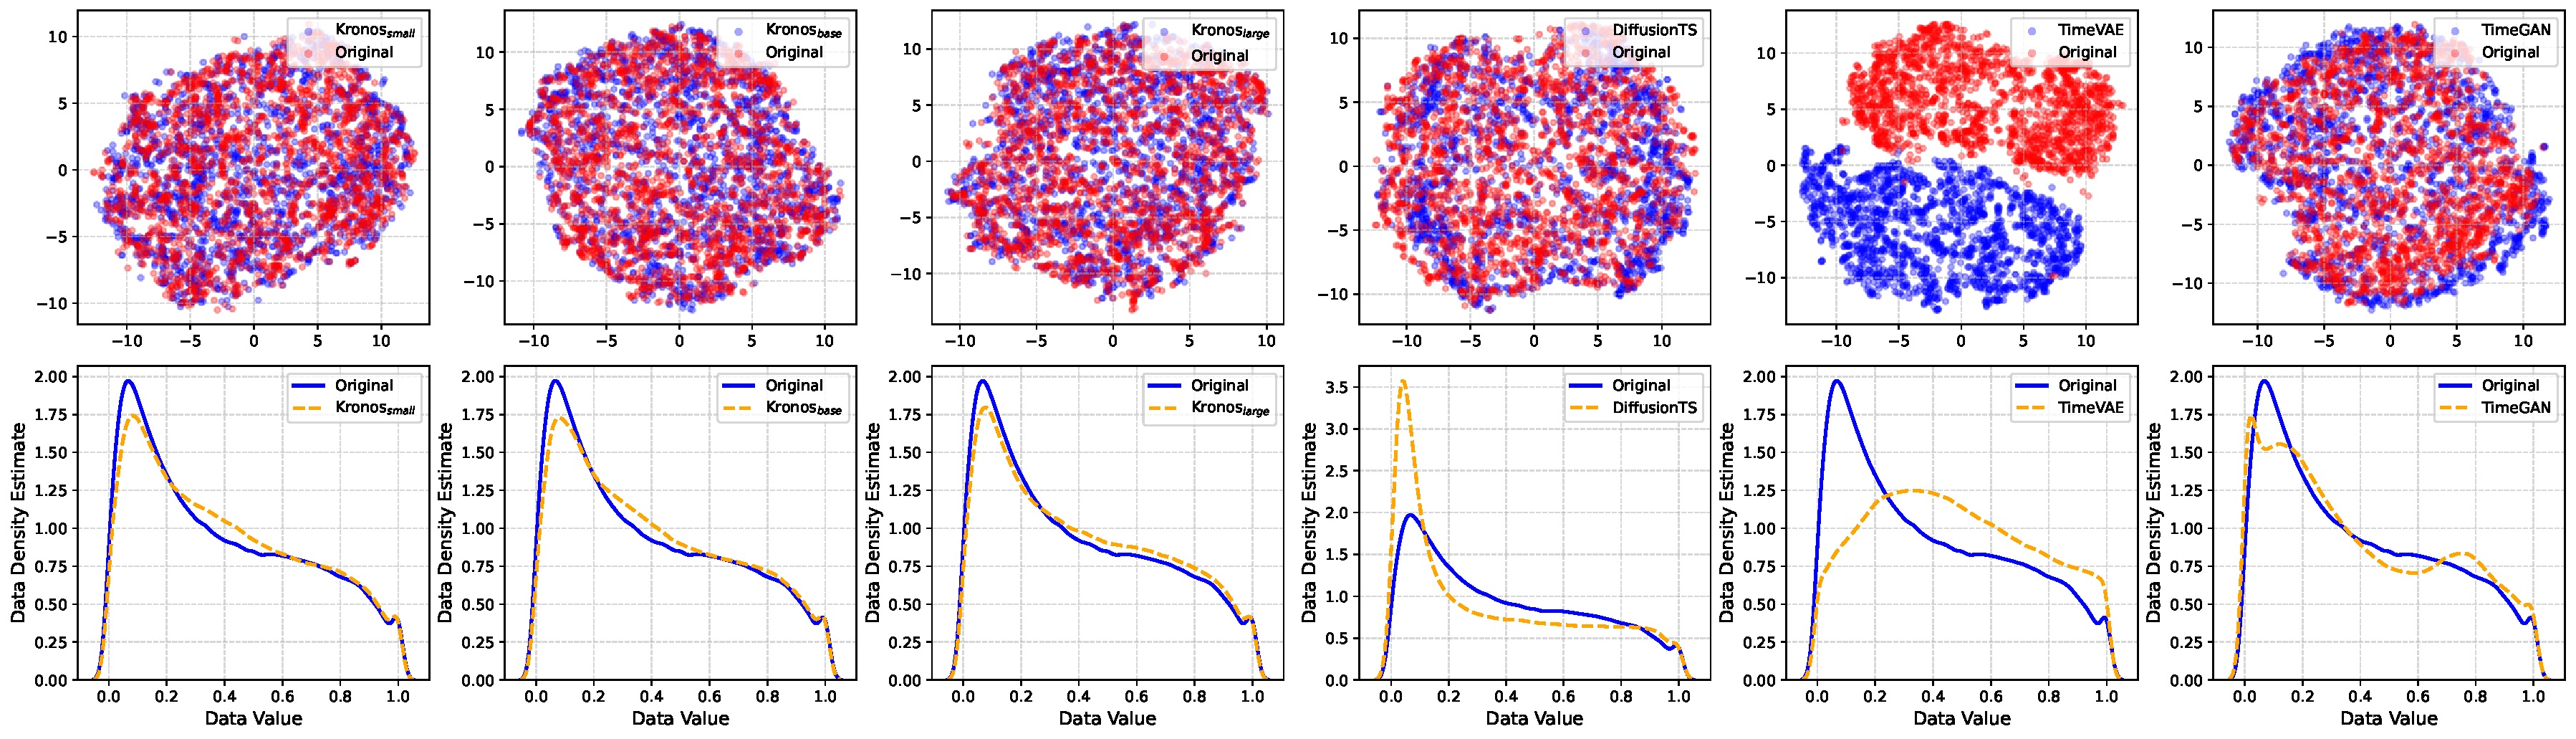
\includegraphics[width=1.0\textwidth]{img/gen_diversity_XSHG_15min.pdf}
    \caption{상하이증권거래소 데이터셋(15분 빈도)에서 생성 모델들의 시각적 비교.
    \textbf{상단 행:} 원본(\textcolor{red}{빨간색}) 데이터와 합성(\textcolor{blue}{파란색}) 데이터의 t-SNE 임베딩.
    \textbf{하단 행:} 원본 데이터와 합성 데이터의 커널 밀도 추정(KDE).}
    \label{fig:gen_diversity_XSHG_15min}
\end{figure*}

금융 K-line 데이터의 기반 모델로서 Kronos의 능력을 종합적으로 평가하기 위해, 우리는 5개의 대표 과제에 걸친 일련의 실험을 설계한다. 이러한 과제들은 예측 및 생성 응용 모두에서 Kronos의 성능을 평가하도록 선정되었으며, 이를 통해 실제 정량 금융 시나리오에서의 다재다능함을 입증한다.

\subsection{실험 설정}

실험 과제는 예측 응용(가격 시계열, 수익률 및 실현 변동성 예측), 생성 능력(합성 K-line 생성), 그리고 실제 적용 가능성을 가늠하기 위한 투자 시뮬레이션을 포괄한다.

엄밀한 비교를 위해, 우리는 25개의 기준 모델로 구성된 포괄적인 모음과 Kronos를 벤치마크한다. 이러한 기준선은 네 가지 서로 다른 패러다임 전반의 최신 기술을 대표하도록 신중히 선정되었다: 사전학습되지 않은 full-shot 모델(예: iTransformer~\cite{liuitransformer}), zero-shot time series foundation model(예: TimeMOE~\cite{xiaoming2025time}), 계량경제학적 변동성 모델(예: GARCH~\cite{bollerslev1986generalized}, 계량경제학의 변동성 예측을 위한 고전적 접근법), 그리고 생성형 시계열 모델(예: DiffusionTS~\cite{yuan2024diffusion}).
과제 세부사항과 기준선은 부록~\ref{sec:exp_setup_details}에 제시되어 있다. 주요 실험 결과의 개요는 그림~\ref{fig:main_result}에 제시되어 있으며, 전체 결과 세부 내역은 부록~\ref{sec:full_exp_results}에 있다.


\subsection{주요 결과}

\subsubsection{예측 과제}
그림~\ref{fig:main_result}(a-c)는 세 가지 예측 과제의 결과를 제시한다. Kronos는 이들 모두에서 일관되게 최첨단 성능을 달성한다. 특히 가격 시계열 예측에서 Kronos는 가장 강력한 TSFM 기준선 대비 RankIC에서 놀라운 93\% 향상을 달성하고, 최고의 사전학습되지 않은 모델 대비 87\%의 이득을 얻는다. 또한 모델 크기가 커질수록 이러한 과제에서의 성능이 일관되게 향상되어, time series foundation model의 scaling laws를 실증적으로 검증한다~\cite{yao2024towards}.


\subsubsection{생성 과제}

확립된 관행~\cite{yoon2019time}에 따라, 우리는 합성 데이터의 품질을 세 가지 관점, 즉 \textit{다양성}, \textit{충실도}, \textit{유용성}에서 평가한다.
\textit{다양성}—생성된 샘플이 실제 데이터의 분포를 얼마나 잘 포괄하는지—을 평가하기 위해, 우리는 두 가지 시각적 방법을 사용한다: t-SNE를 사용해 원본 및 합성 데이터를 2D 공간에 투영하고, 커널 밀도 추정(KDE)을 통해 이들의 분포를 비교한다. 그림~\ref{fig:gen_diversity_XSHG_15min} 및 부록~\ref{sec:full_exp_results}에 나타난 바와 같이, t-SNE 플롯은 Kronos의 합성 데이터가 원본 데이터 공간과 더 잘 겹침을 보여주며, KDE 플롯은 분포의 더 높은 유사성을 확인해 준다.

정량적 평가를 위해, 우리는 판별 점수를 사용하여 \textit{충실도}(즉, 데이터 현실성)를 평가한다. 이 점수는 분류기가 원본 샘플과 합성 샘플을 구별하는 것이 얼마나 어려운지를 측정한다. 또한 Train-on-Synthetic, Test-on-Real (TSTR) 프로토콜을 통해 \textit{유용성}(다운스트림 모델 학습을 위한 합성 데이터의 효과)을 평가한다. 여기서는 예측 모델을 합성 데이터로 학습하고, 실제 데이터로 구성된 테스트 세트에서 그 결과 IC와 RankIC를 평가한다. 그림~\ref{fig:main_result}(d)에 나타난 바와 같이, Kronos는 \textit{충실도}와 \textit{유용성} 모두에서 최고의 성능을 달성한다. 이러한 우수성은 모델 크기가 커질수록 또한 강화된다.

\subsubsection{투자 시뮬레이션}
현실적인 투자 시나리오에서 Kronos의 성능을 검증하기 위해, 우리는 각 모델의 예측 신호로 순위를 매긴 상위-$k$ 종목으로 포트폴리오를 구성하여 중국 A-shares 시장에서 long-only 투자 전략을 시뮬레이션한다.
그림~\ref{fig:main_result}(e)에 나타난 바와 같이, Kronos는 모든 다른 기준선을 능가하며 가장 높은 Annualized Excess Return (AER)과 Information Ratio (IR)를 달성한다. 이는 모델이 우수한 예측 정확도를 실질적인 투자 수익으로 효과적으로 전환할 수 있음을 보여준다.

\subsection{제거 연구}

우리는 핵심 설계 선택을 검증하기 위해 두 가지 질문에 초점을 맞춘 제거 연구를 수행한다: (Q1) 다른 대안들과 비교한 우리의 모델링 패러다임의 효과성, 그리고 (Q2) 어휘 크기의 영향. tokenizer에 대한 추가 제거 연구는 부록~\ref{sec:tokenizer_ablation}에 제공된다.

\noindent\textbf{모델링 패러다임 분석.}
Q1을 다루기 위해, 우리는 비슷한 파라미터 수를 유지하면서 예측 공간과 목적 함수가 다른 변형들과 Kronos를 비교한다. (표~\ref{tab:ablation_study_refined}).
이러한 아키텍처 변형에 대한 자세한 설명은 부록~\ref{sec:ablation_baselines}에 제공된다. 우리는 두 가지 연속 공간 모델, 즉 \textit{Direct-AR}(MSE를 사용하는 회귀 기준선)과 \textit{Prob-AR}을 테스트한다. 확립된 연구~\cite{yao2024towards}에 따라, \textit{Prob-AR}은 heavy-tailed 데이터 분포를 더 잘 모델링하기 위해 Student-t 혼합 분포를 사용한다. 결과는 우리의 이산 공간 모델들이 이러한 연속형 대안들을 현저히 능가함을 보여준다. 또한 서브토큰을 동시에 예측하는 변형인 \textit{Kronos-Parallel}이 우리의 순차적 접근법보다 성능이 낮다는 점도 발견했으며, 이는 서브토큰 의존성을 모델링하는 것의 중요성을 보여준다.
이러한 발견은 이 영역에서 우리의 이산적이고 순차적인 모델링 프레임워크가 더 효과적인 접근법임을 검증한다.



\begin{figure}[t!]
    \centering
    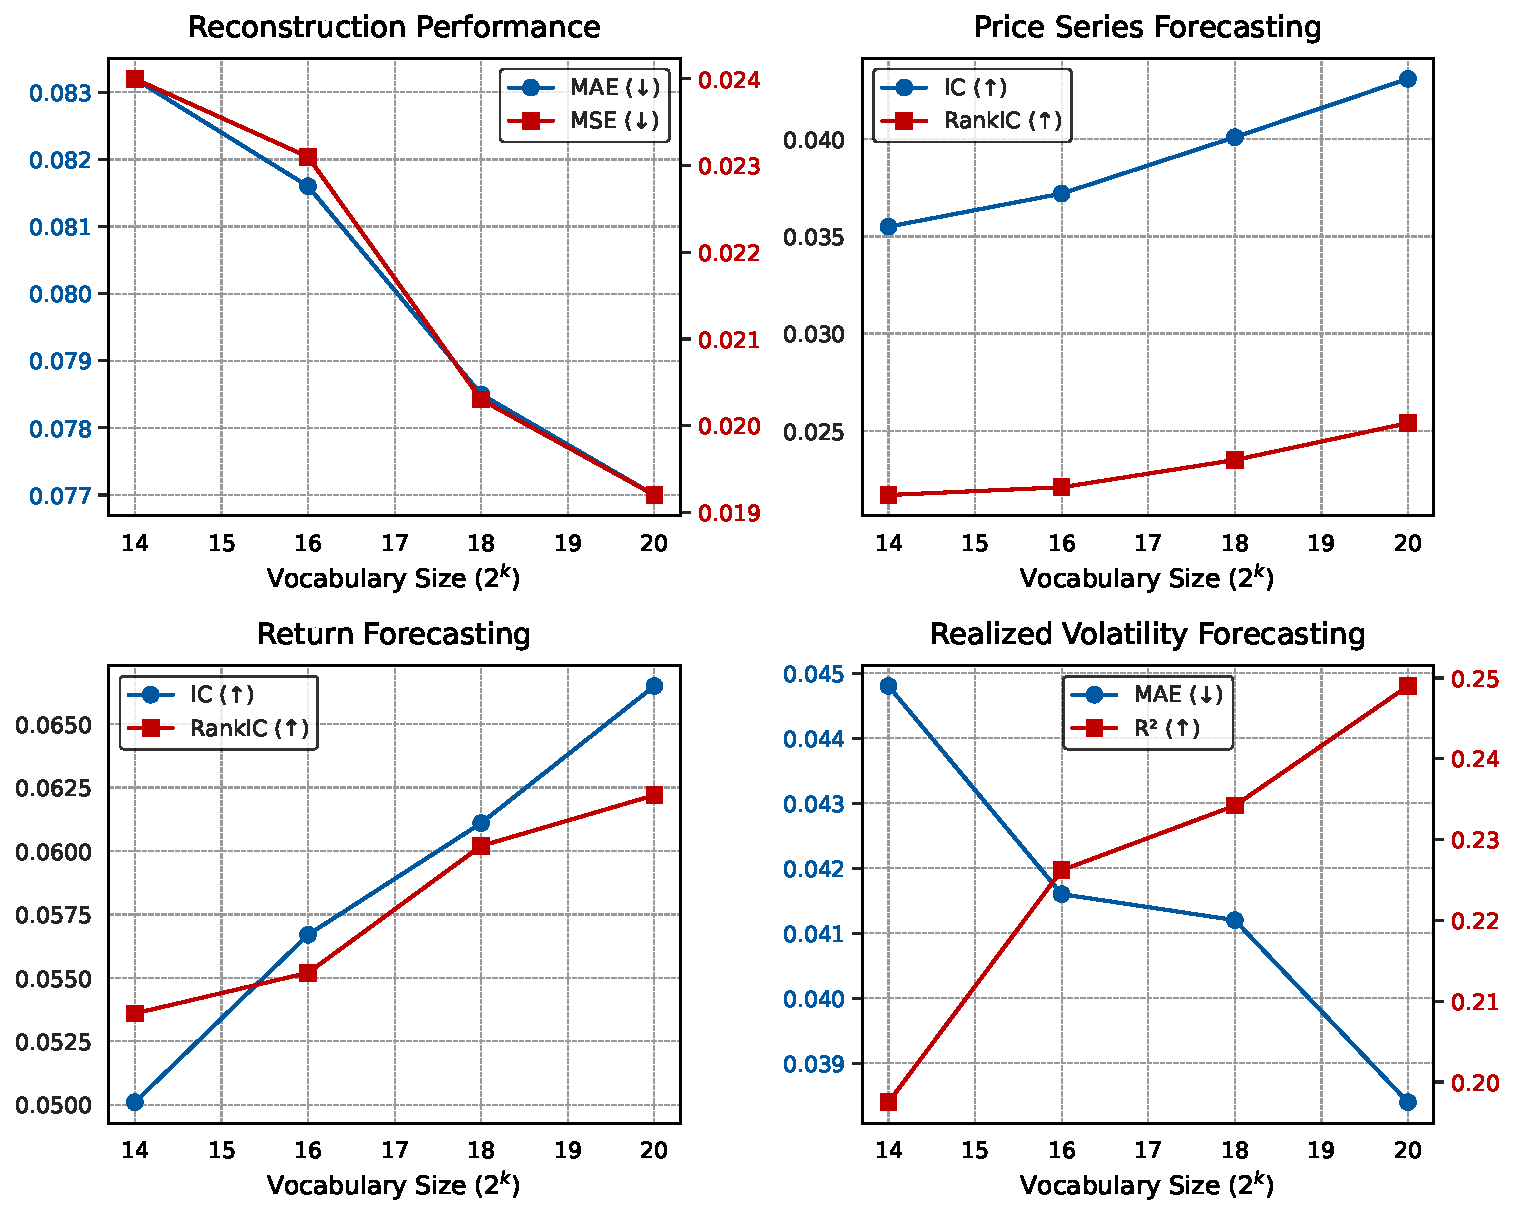
\includegraphics[width=1.0\columnwidth]{img/model_performance_vs_vocab_size.pdf}
    \caption{어휘 크기가 모델 성능에 미치는 영향. 우리는 어휘 크기가 증가함에 따라 재구성 품질과 다운스트림 예측 성능을 플롯한다.
    }
    \label{fig:vocab_size}
\end{figure}

\noindent\textbf{어휘 크기의 영향.}
Q2에 답하기 위해, 우리는 어휘 크기가 모델 성능에 어떤 영향을 미치는지 조사한다. 그림~\ref{fig:vocab_size}에 나타난 바와 같이, 어휘 크기를 늘리면 재구성 품질과 예측 정확도가 모두 향상된다. 더 큰 어휘는 더 세밀한 표현을 제공하여 양자화 오차를 줄인다. 결정적으로, 이렇게 향상된 표현 정밀도는 더 나은 예측 결과로 이어진다. 이 발견은 LFQ 및 BSQ와 같은 양자화 기법에서 더 큰 어휘가 생성 품질 향상으로 이어지는 것으로 나타난 비디오 생성 분야의 관찰과 일치한다~\cite{zhao2024image,yu2023language}.


\begin{figure}[t!]
    \centering
    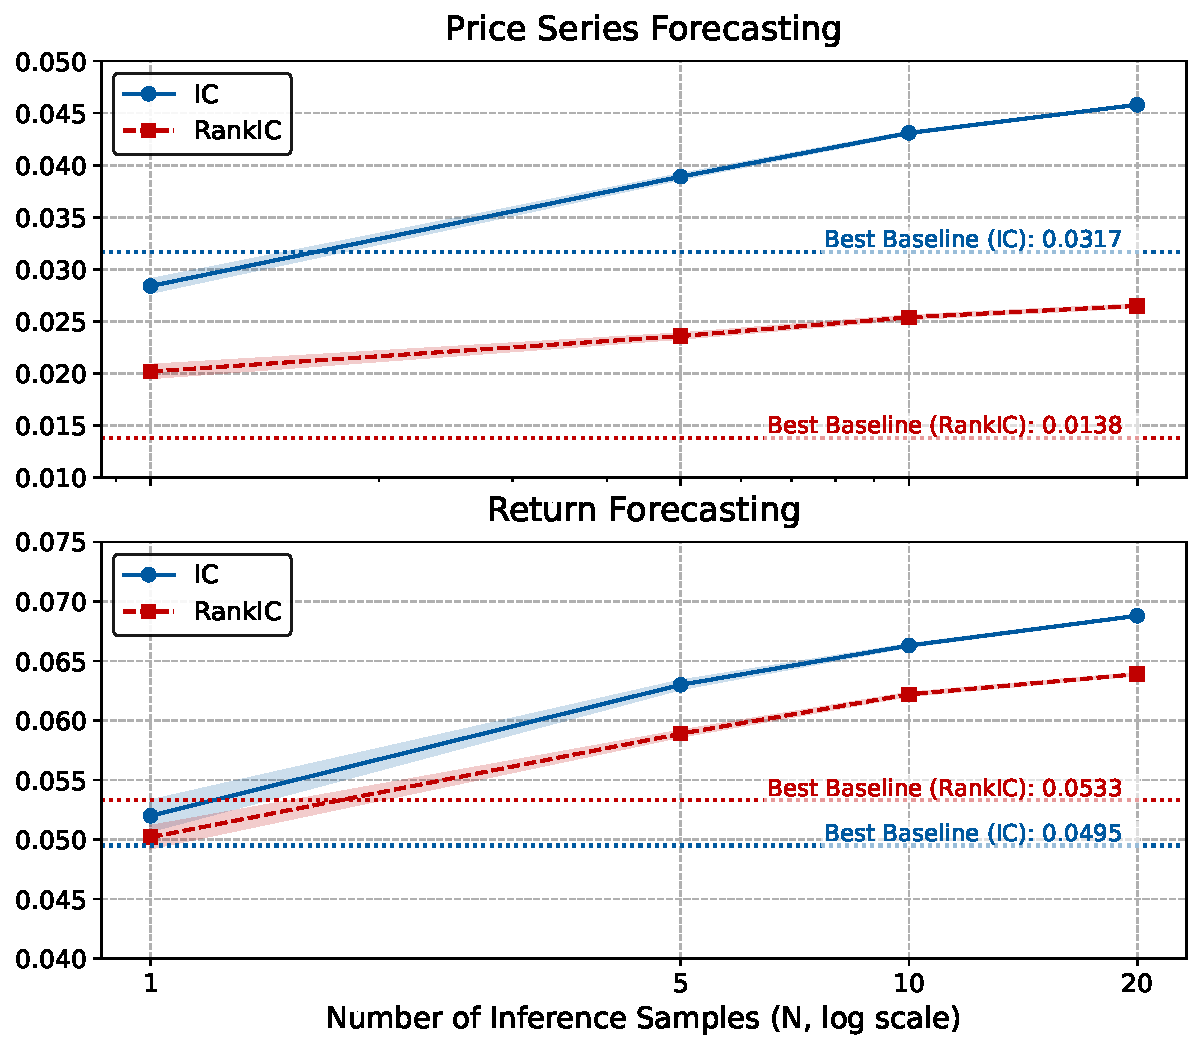
\includegraphics[width=1.0\columnwidth]{img/mc_sampling_performance.pdf}
    \caption{추론 샘플 수(N)가 예측 성능에 미치는 영향. 선은 서로 다른 무작위 시드를 사용한 5회 실행의 평균 성능을 나타내며, 음영 영역은 표준편차를 나타낸다.
    % 추론 샘플 크기(N)가 예측 성능에 미치는 영향. 평균(선)과 표준편차(음영)는 서로 다른 무작위 시드를 사용한 5회 실행에서 계산된다.
    }
    \label{fig:inference_sample}
\end{figure}

\subsection{테스트 시점 스케일링}
\label{sec:test_time_scaling}

우리의 확률적 생성 프레임워크의 주목할 만한 장점은 모델을 재학습하지 않고도 추론 시점에 예측 정확도를 향상시킬 수 있다는 점이다. 확률적 샘플링을 활용함으로써 Kronos는 동일한 맥락에서 여러 개의 서로 다른 미래 궤적을 생성할 수 있다. 우리는 샘플링된 경로 수를 늘려가며 그 결과를 평균함으로써 이러한 예측들을 앙상블하는 효과를 조사한다. 그림~\ref{fig:inference_sample}은 샘플 수의 함수로서 예측 과제 성능을 제시한다. 결과는 앙상블에 더 많은 샘플이 포함될수록 IC와 RankIC 모두에서 일관된 향상이 나타남을 보여준다. 여러 경로에 걸친 평균은 생성 과정에 내재한 확률성을 완화하고 예측 분산을 줄여, 더 견고하고 안정적인 추정치를 산출한다. 이 능력은 실무자가 추론 시 계산 비용과 원하는 예측 정확도 수준 사이의 균형을 맞출 수 있게 하는 절충점을 제공한다.
